% CVPR 2022 Paper Template
% based on the CVPR template provided by Ming-Ming Cheng (https://github.com/MCG-NKU/CVPR_Template)
% modified and extended by Stefan Roth (stefan.roth@NOSPAMtu-darmstadt.de)

\documentclass[10pt,twocolumn,letterpaper]{article}

%%%%%%%%% PAPER TYPE  - PLEASE UPDATE FOR FINAL VERSION
%\usepackage[review]{cvpr}      % To produce the REVIEW version
%\usepackage{cvpr}              % To produce the CAMERA-READY version
\usepackage[pagenumbers]{cvpr} % To force page numbers, e.g. for an arXiv version

% Include other packages here, before hyperref.
\usepackage{graphicx}
\usepackage{amsmath}
\usepackage{amssymb}
\usepackage{booktabs}
\usepackage{makecell}


% It is strongly recommended to use hyperref, especially for the review version.
% hyperref with option pagebackref eases the reviewers' job.
% Please disable hyperref *only* if you encounter grave issues, e.g. with the
% file validation for the camera-ready version.
%
% If you comment hyperref and then uncomment it, you should delete
% ReviewTempalte.aux before re-running LaTeX.
% (Or just hit 'q' on the first LaTeX run, let it finish, and you
%  should be clear).
\usepackage[pagebackref,breaklinks,colorlinks]{hyperref}


% Support for easy cross-referencing
\usepackage[capitalize]{cleveref}
\crefname{section}{Sec.}{Secs.}
\Crefname{section}{Section}{Sections}
\Crefname{table}{Table}{Tables}
\crefname{table}{Tab.}{Tabs.}


%%%%%%%%% PAPER ID  - PLEASE UPDATE
\def\cvprPaperID{*****} % *** Enter the CVPR Paper ID here
\def\confName{CVPR}
\def\confYear{2022}


\begin{document}

%%%%%%%%% TITLE - PLEASE UPDATE
\title{Elephace: Elephant Re-identification Using Deep Learning}

\author{First Author\\
Institution1\\
Institution1 address\\
{\tt\small firstauthor@i1.org}
% For a paper whose authors are all at the same institution,
% omit the following lines up until the closing ``}''.
% Additional authors and addresses can be added with ``\and'',
% just like the second author.
% To save space, use either the email address or home page, not both
\and
Second Author\\
Institution2\\
First line of institution2 address\\
{\tt\small secondauthor@i2.org}
}
\maketitle

%%%%%%%%% ABSTRACT
\begin{abstract}

The goal of our project is to build vision model to re-identify elephants using their images. This model will be used by researchers to track elephant movement pattern in zoos and sanctuaries. 
This non-invasive way of recognizing elephants is better than capturing and attaching devices to them which requires human intervention. Manually identifying elephants from images is a time-consuming process and a good automated model is essential. We have built an elephant re-identification model using three deep learning methods and performed experiments to identify the best parameters for the model. Our primary dataset (aka zoo dataset) provided by Prof. Chusyd. We have built a classification model to classify an image into one of the known elephant categories. With ResNet50 as the backbone and our primary dataset, this model's top-1 accuracy was 99.71\%. We aimed to recognize elephants with as few images as possible in our next approach, therefore we constructed a few shot learning model. Using just 3 images per class we obtained top-1 accuracy of 81\% and top-3 accuracy of 92\% on our primary dataset. The performance of few shot on more complex wild elephants dataset was not as good as zoo elephants so we moved to training Siamese network using triple loss (ala FaceNet). With the best hyperparameter choices, we got validation rate of 0.585 at false acceptance rate of 0.01.



\end{abstract}

%%%%%%%%% BODY TEXT
\section{Introduction}
\label{sec:intro}

Re-identification of animals is necessary for biodiversity monitoring and ecological research projects. Biologists and anthropologists need animal tracking to monitor their health, behavior, group dynamics and variation of population over time [Deb, Debayan, et al.]. Biodiversity development and health information is highly valuable for assessing the environmental effect and necessary steps required to preserve the ecosystems.

Animal tracking can be performed by using a device that is attached to the animal. This technique requires human intervention and it is intrusive. It requires capturing animals which can be dangerous and also disruptive for an animal's wild habitat [Deb, Debayan, et al.]. Another method of tracking animals is by capturing the images and re-identifying animals from those images. The re-identification performed manually can be a time consuming process as multiple and vast numbers of images need to be analyzed. This re-identification requires domain knowledge about the particular species and also its prone to biases related to human judgment [Schneider, Stefan, et al.].

Automated re-identification of animals provides a better solution to animal tracking without involving disruptive techniques and human errors. There has been ongoing research to extend human face recognition and identification techniques to animal identification using deep learning. There are many challenges while building a state of the art animal re-identification and classification model. These challenges arise due to similar looking animals and very small distinctive features like body size, scars and marks, coloring, etc [Körschens, et al.]. Apart from this, these features could also change over time. For example in the case of elephants, it could lose a tusk and a hole in the ear may become a rip [Körschens, et al.]. Other challenges are variations in image captured such as occlusion, varying viewpoints, different poses and angles of the animal in an image that affect the detection of distinctive features. For example in the case of elephants the feature might not be clearly visible in images because of mud on their bodies or the angle and movement [Körschens, et al.].

In this project, we have build a model for elephant re-identification system using bounding box detection architecture for bounding box predictions followed by multiple deep learning network architectures for elephant re-identification.

\begin{figure}[t]
  \centering
  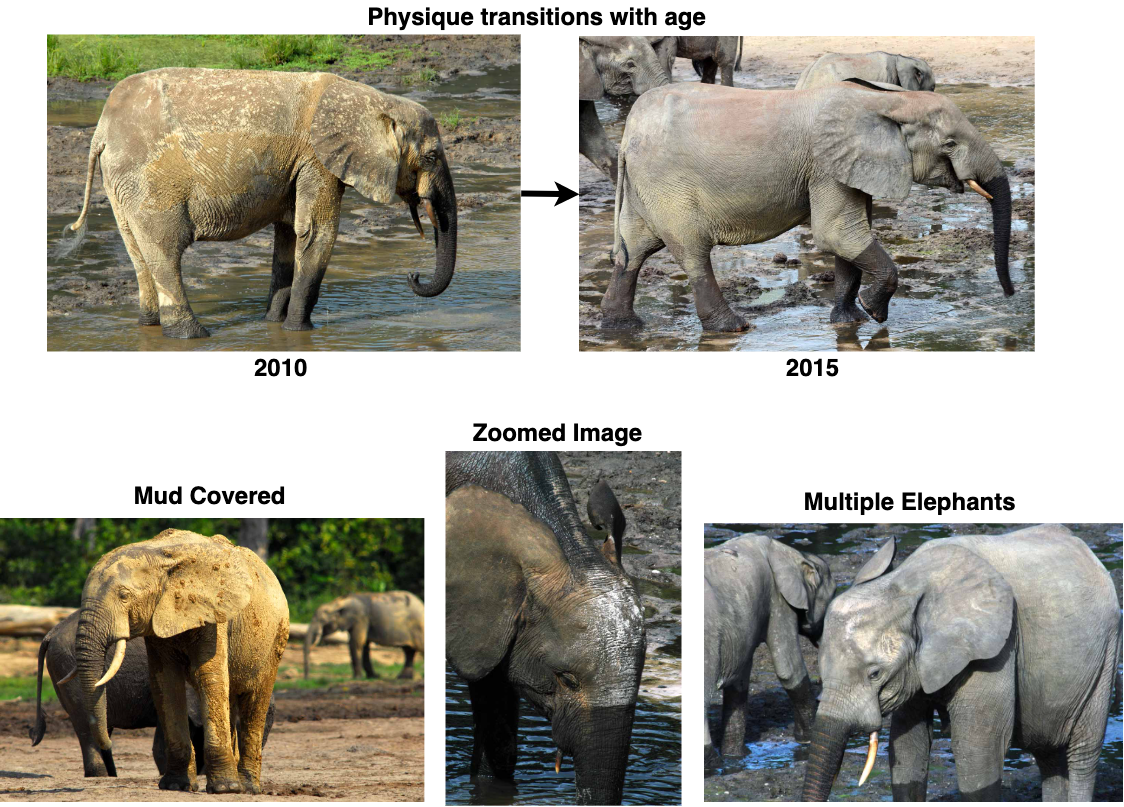
\includegraphics[scale=0.2]{challenges}
   \caption{Clockwise: Elephant Physique transitions with age, Elephant covered in mud, zoomed image, multiple animals in an image}
   \label{fig:challenges}
\end{figure}


%-------------------------------------------------------------------------

\section{Background and related work}
\label{sec:backgoround}

In the context of animal re-identification, various works have used custom feature engineering and classical computer vision techniques. Recently there has been some work on using the advanced and already mature human face recognition techniques e.g. FaceNet, DeepFace for animal recognition and identification tasks.

[Korschens et al] used a pre-trained YOLO network for bounding box predictions to automatically locate an elephant's heads in images using pre pre-trained YOLO network.Used a human in the loop approach to select the best bounding box and then the bounding box is cropped and fed into a pre-trained ResNet 50 for feature extraction from the middle layer followed by pooling. PCA is used to reduce the number of features and then SVM is used for classification. To improve the accuracy, results of multiple images of the same elephant are aggregated by averaging the class wise confidence. The Top 1 accuracy for classification is 56\% and 74\% with two image aggregation. For the same task but using traditional methods [Ardovini et al][Schneider review] - performed re-identification of elephants using multi-curve matching technique and achieved top-1 accuracy for 75\%.

For primate re-identification [Debayan Deb et al] implemented a variation of a sphereface deep recognition to build embeddings of faces which then can be compared using similarity functions. Instead of using an object detection network to identify the faces, they manually annotated landmarks to align the faces. They achieved a closed set accuracy of 75.82\% on the chimpanzee dataset.

For identification of giant pandas, [Jin Hou et al] used significant data augmentation and trained a VGGnet for classification tasks. They were able to accurately identify 90\% of panda individuals.

For the difficult task of Nyala identification, [Zyl et al] implemented an end to end system consisting of Faster R-CNN model for bounding box detection and then siamese network using ResNet-152 backbone for image embedding. Their top1 accuracy for zebra dataset is 74.1\% and top-10 accuracy of 85\% for Nyala animal identification.

[Freytag et al] uses matrix logarithm transformation on bilinear pooling to increase the discriminability of features in Alexnet and VGGfaces networks. Using these techniques, they achieved the state of the art for chimpanzee faces classification. For a similar task, Gorilla faces classification [Brust et al] uses YOLO and R-CNN for bounding box detention along with AlexNet for feature extraction upon which they used SVM for class label prediction.

%-------------------------------------------------------------------------


\section{Methods}
\label{sec:methods}

\subsection{Elephant Detection and Extraction}

In order to accurately identify elephant in an image, it is essential to isolate it from surrounding which might contain other elephants, animals or people. For this reason, a pre-trained object detection model is used to obtain bounding boxes for all the elephants in the image. If there are multiple elephants detected, then the elephant with the bounding box of largest area is considered to be the subject and extracted.

Yolov4 \cite{yolov4}, Faster R-CNN Inception ResNet V2 1024x1024 \cite{fasterrcnn}, and SSD MobileNet v2 320x320 \cite{ssdnet} pre-trained models were tried to detect and get bounding boxes for the elephants. The Yolov4 pretrained model is obtained from \cite{tf2yolov4} and Faster R-CNN Inception ResNet V2 1024x1024 and SSD MobileNet v2 320x320 are obtained from Tensorflow Object detection zoo \cite{tensorflowzoo}. It is found that for these datasets, bounding boxes obtained from Yolov4 often times did not include the head of the elephant see fig:\ref{fig:boundingbox_comparison}. For this reason, Faster R-CNN and SSD MobileNet are used to extract the elephant for the next phase.

\begin{figure}[t]
  \centering
  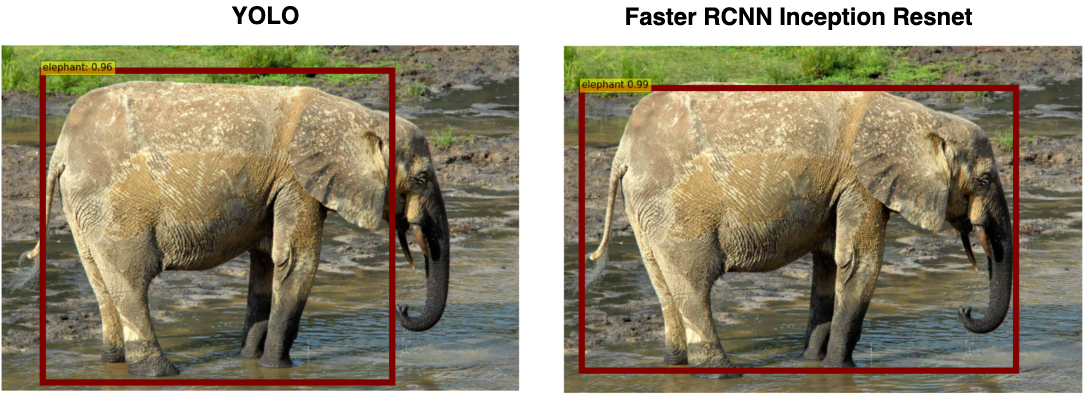
\includegraphics[scale=0.2]{Bounding_box}
   \caption{Bounding Box Detected by Yolov4 and Faster RCNN Inception ResNet V2}
   \label{fig:boundingbox_comparison}
\end{figure}

\begin{figure}[t]
  \centering
  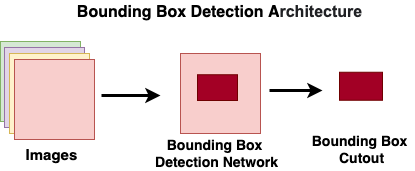
\includegraphics[scale=0.35]{boundingbox_network}
   \caption{Elephant Bounding Box Detection}
   \label{fig:boundingbox_network}
\end{figure}

To re-identify an elephant given some of its images we consider three approaches - classification, few-shot recognition, and Siamese network for similarity measurements.

\subsection{Classification}

When the problem of re-identification is posed as a classification, the model is trained with labelled images of elephants. Both the train and validation sets will consist of disjoint images of the same elephant and the model has to learn the discriminative features and use them to predict the label of elephant images from the validation set. Our classification model consists of a pre-trained CNN as a backbone to provide the image embeddings and a couple of fully connected layers with softmax to classify the images into one of the elephants from the train set. Cross-entropy loss along with L2 regularization for the fully connected layers is used for training the model.


\subsection{Few Shot Learning}

When there are only a few images available per elephant, the train set used for classification becomes imbalanced and learning becomes difficult. To solve this problem few shot learning paradigm is utilized, where image embeddings from a pre-trained CNN of known images are compared with the embeddings of unknown images using a suitable similarity metric \cite{fewshotclassification}. 

Using a pre-trained CNN, the image embeddings are obtained. 

Support set, query set

query set image embedding, dot product, with mean embedding of the support set

normalized embeddings

softmax over the dot product results of all comparisons

finetune
- initial value of W
- entropy regularization
- cosine similarity instead of dot product

$$
w_{S_k} = \sum_{s \in S_k} \cfrac{ \lVert f(x_s) \rVert}{  | S | }
$$

$$
z_{S_k}^{(q)} = \cfrac{w_{S_k}^T \lVert f(x_q) \rVert}{\lVert w_{S_k} \rVert} + b_{S_k}
$$

$$
\hat{y}^{(q)} = softmax(z^{(q)})
$$

$$
\mathcal{L} = \sum_{j}\sum_{i} (y_i^{(j)} log(\hat{y}_i^{(j)}) + \hat{y}_i^{(j)} log({\hat{y}_i^{(j)}}))
$$

where $y_i^{(j)}$ and $\hat{y}_i^{(j)}$ is the $i^{th}$ component of the true label and predicted labels of $j^{th}$ example respectively.

The ideas above are from \cite{fewshotlectures}, \cite{fewshotbaseline}, \cite{fewshotmetabaseline}


\begin{figure}[t]
  \centering
  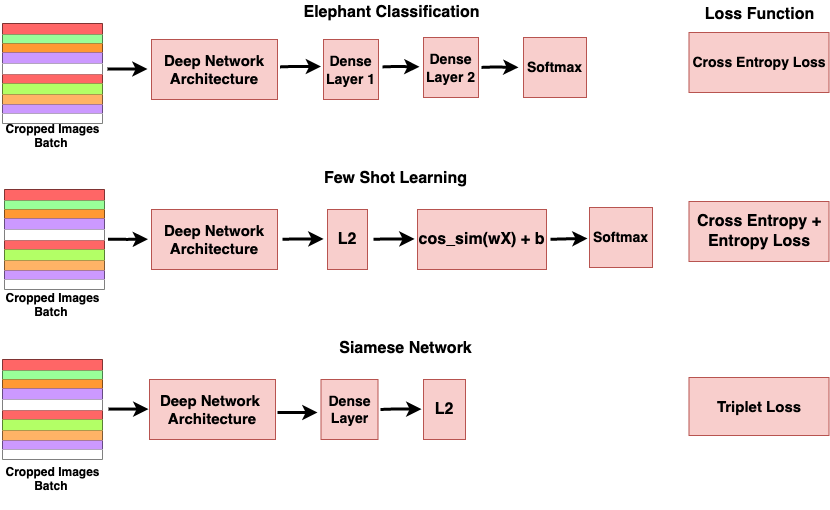
\includegraphics[scale=0.275]{reidentification_network}
   \caption{Elephant re-identification architectures}
   \label{fig:reidentification_network}
\end{figure}

\subsection{Siamese Network}

Facenet paper

triplet loss

$$
\mathcal{L} = \sum_{i}^N \Big[ \lVert f(x_i^a) - f(x_i^p)\rVert_2^2 - \lVert f(x_i^a) - f(x_i^n)\rVert_2^2  + \alpha \Big]
$$

batchall

batch hard

hard positive: $x_i^P = \text{argmax}_{x_i^p}  \lVert f(x_i^a) - f(x_i^p)\rVert_2^2$

hard negative: $x_i^N = \text{argmin}_{x_i^n}  \lVert f(x_i^a) - f(x_i^n)\rVert_2^2$

batch partial hard

%-------------------------------------------------------------------------



\section{Experiments and Results}
\label{sec:expresults}

Table \ref{tab:exp} shows experiments performed on all three models:

\begin{table}[h!]
  \begin{center}
    \begin{tabular}{ c | c | c} 
      \textbf{Classification} & \textbf{Few Shot} & \textbf{Siamese}\\
      \hline
      \makecell{RestNet50,  \\ InceptionV3} & \makecell{ RestNet50, \\ InceptionV3} & \makecell{RestNet50, \\ InceptionV3 }\\
       \hline
      \makecell{Image \\ Augmentation}  & \makecell{Image \\Augmentation} & \makecell{Image \\ Augmentation}\\
      \hline
      Finetuning  & Finetuning & Embedding size\\
      \hline
        & Support set size & Triplet loss margin\\
     \hline
     	& & Triplet loss strategy\\
     \hline
	& & \makecell{Optimizer: \\ Adam, SGD}\\
     \hline
      	& & Aspect Ratio\\
    \end{tabular}
  \caption{Model Experiments}
  \label{tab:exp}
  \end{center}
\end{table}

\subsection{Elephant Classification}

For elephant classification model, we used two backbone models of ResNet50 and InceptionV3. We trained the model using these two backbone models along with image augmentation and fine-tuning.We found that both the model performed well on zoo elephants dataset with top-1 accuracies of 0.9971 and 0.979 respectively. This model did not perform well on wild dataset with top-1 accuracies of 0.21 and 0.16 respectively. The top-1, 3, and 5 accuracies for both zoo and wild dataset are shown in Table 


\subsection{Few Shot Learning}

In Few shot learning, we have used two backbone architectures of ResNet50 and InceptionV3.Both these model performed well on zoo elephants and didn't perform well on wild elephants. 
Next, we trained the models with and without image augmentation.Image augmentations consisted of left-right flip, small random changes to saturation and hue as shown in figure \ref{fig:augmentation}. We observed that performing image augmentation improved the accuracy by 17\%. We experimented with preserving the aspect ratio of images by padding them as shown in figure \ref{fig:image_padding} but it caused degradation of performance. We fine-tuned the model with entropy regularization and observed that the accuracy improved by 35\%. Graph \ref{fig:finetune_graph} shows the performance of model for various support set with and without fine-tuning implementation. For few shot learning, we have used support set size of 1, 2, 3, 5, 7, and 9. Graph \ref{fig:few_shot_graph} shows the Top-1 accuracy for model for various support sizes. It was observed that the support size of just 3 performed well with top-1 accuracy of about 81\% on zoo dataset. Furthermore, the top-1 accuracy of 99\% was achieved with the support set of 7. 

\begin{figure}[t]
  \centering
  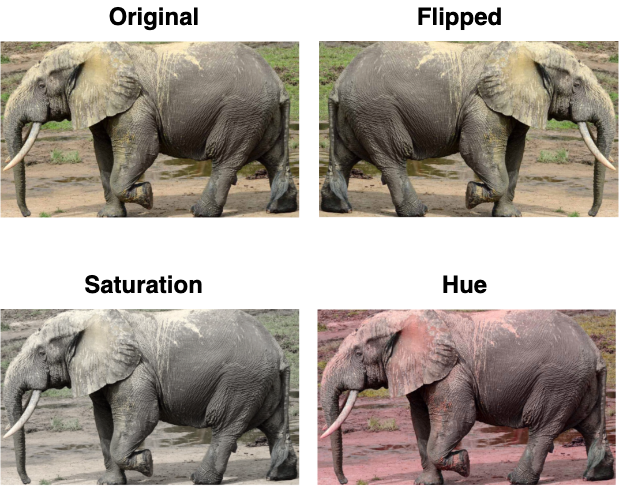
\includegraphics[scale=0.37]{augmentation}
   \caption{Image augmentations performed are right-left flip, saturation and hue changes}
   \label{fig:augmentation}
\end{figure}

\begin{figure}[t]
  \centering
  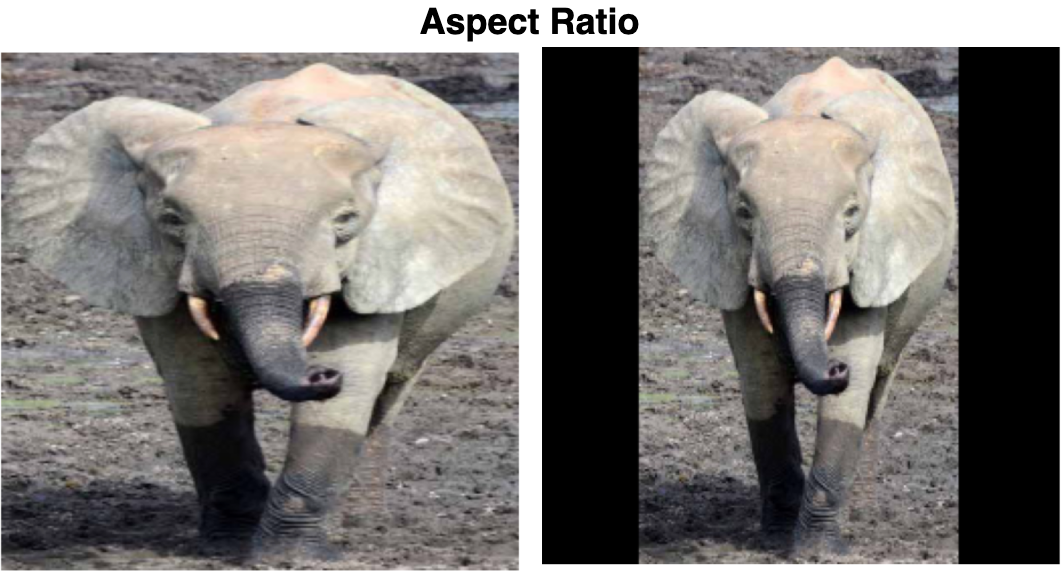
\includegraphics[scale=0.23]{image_padding}
   \caption{Image Padding: To preserve Aspect Ratio}
   \label{fig:image_padding}
\end{figure}

\begin{figure}[t]
  \centering
  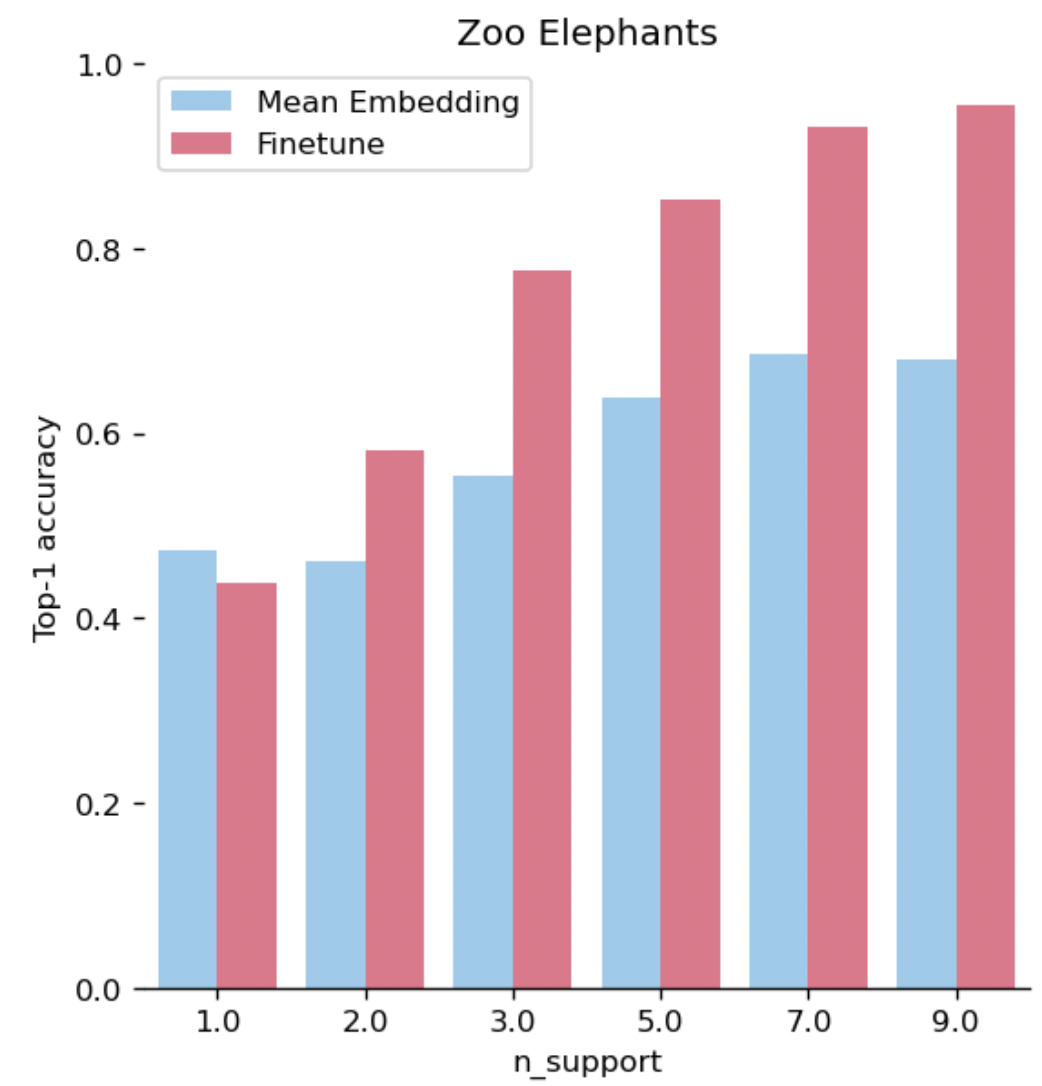
\includegraphics[scale=0.50]{finetune_graph}
   \caption{Fine-tuning with entropy regularization}
   \label{fig:finetune_graph}
\end{figure}

\begin{figure}[t]
  \centering
  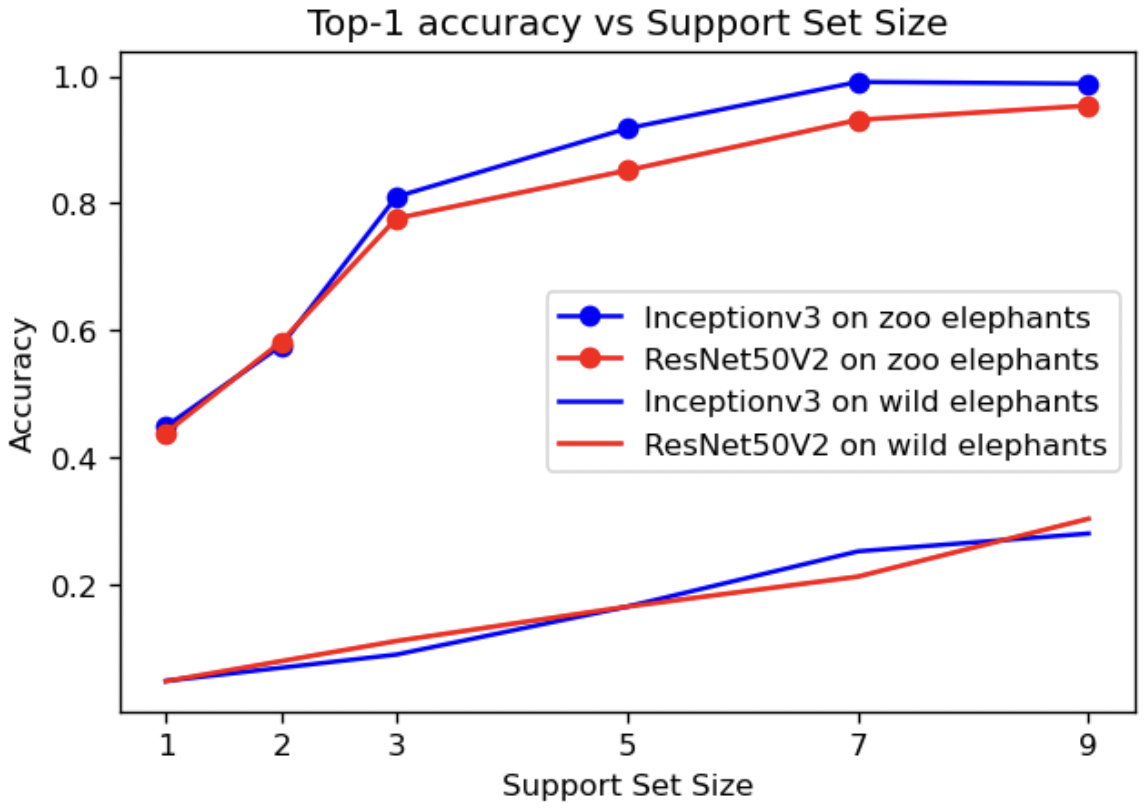
\includegraphics[scale=0.45]{few_shot_graph}
   \caption{Graph of Top-1 Accuracy with support set size}
   \label{fig:few_shot_graph}
\end{figure}

\subsection{Siamese Network}

In Siamese Network, we have  experimented with two backbone architectures of ResNet50 and InceptionV3 along with image augmentation. While training siamese network, we experimented with various triplet loss margins of 0.2, 0.5, 0.75 and selected margin of 0.5. We used triplet loss strategies of batch triplet loss and hard triplet loss. We observed the model performance using two optimizer: Adam and SGD and chose Adam optimizer. The model's performance was then tested with different embedding sizes: 64, 128 and 256, with the 256 embedding size providing the best results. Table \ref{} shows the VAL rate for embedding sizes of 64, 128 and 256.

%-------------------------------------------------------------------------

\section{Discussion}
\label{sec:discussion}





%-------------------------------------------------------------------------


\section{Conclusion}
\label{sec:conclusion}






%-------------------------------------------------------------------------


\begin{thebibliography}{99}

\bibitem{yolov4}
	Bochkovskiy, Alexey, Chien-Yao Wang, and Hong-Yuan Mark Liao. "Yolov4: Optimal speed and accuracy of object detection." arXiv preprint arXiv:2004.10934 (2020).
	
\bibitem{fasterrcnn}
	Ren, Shaoqing, et al. "Faster r-cnn: Towards real-time object detection with region proposal networks." Advances in neural information processing systems 28 (2015).
	

\bibitem{ssdnet}
	Liu, Wei, et al. "Ssd: Single shot multibox detector." European conference on computer vision. Springer, Cham, 2016.


\bibitem{Deb}
	Deb, Debayan, et al. "Face recognition: Primates in the wild." 2018 IEEE 9th International Conference on Biometrics Theory, Applications and Systems (BTAS). IEEE, 2018. 


\bibitem{Korschens}
	Korschens, Matthias, Bjorn Barz, and Joachim Denzler. "Towards automatic identification of elephants in the wild." arXiv preprint arXiv:1812.04418 (2018). 


\bibitem{Freytag}
	Freytag, Alexander, et al. "Chimpanzee faces in the wild: Log-euclidean CNNs for predicting identities and attributes of primates." German Conference on Pattern Recognition. Springer, Cham, 2016. 


\bibitem{Brust}
	Brust, Clemens-Alexander, et al. "Towards automated visual monitoring of individual gorillas in the wild." Proceedings of the IEEE International Conference on Computer Vision Workshops. 2017. 


\bibitem{Zyl}
	Van Zyl, Terence L., Matthew Woolway, and B. Engelbrecht. "Unique animal identification using deep transfer learning for data fusion in siamese networks." 2020 IEEE 23rd International Conference on Information Fusion (FUSION). IEEE, 2020. 


\bibitem{Hou}
	Hou, Jin, et al. "Identification of animal individuals using deep learning: A case study of giant panda." Biological Conservation 242 (2020): 108414. 


\bibitem{Elpephants}
	Korschens, Matthias, and Joachim Denzler. "Elpephants: A fine-grained dataset for elephant re-identification." Proceedings of the IEEE/CVF International Conference on Computer Vision Workshops. 2019. 




\bibitem{SchneiObject}
	Schneider, Stefan, Graham W. Taylor, and Stefan Kremer. "Deep learning object detection methods for ecological camera trap data." 2018 15th Conference on computer and robot vision (CRV). IEEE, 2018.



\bibitem{SchneiReidentify}
	Schneider, Stefan, et al. "Past, present and future approaches using computer vision for animal re‐identification from camera trap data." Methods in Ecology and Evolution 10.4 (2019): 461-470. 

\bibitem{Facenet}
	Schroff, Florian, Dmitry Kalenichenko, and James Philbin. "Facenet: A unified embedding for face recognition and clustering." Proceedings of the IEEE conference on computer vision and pattern recognition. 2015. 


\bibitem{Koch}
	Koch, Gregory, Richard Zemel, and Ruslan Salakhutdinov. "Siamese neural networks for one-shot image recognition." ICML deep learning workshop. Vol. 2. 2015. 
 
\bibitem{tensorflowzoo}
	Tensorflow Object Detection Zoo: \url{https://github.com/tensorflow/models/blob/master/research/object_detection/g3doc/tf2_detection_zoo.md}

\bibitem{tf2yolov4}
	\url{https://github.com/sicara/tf2-yolov4}

\bibitem{fewshotclassification}
	Chen, Liu, Kira, Wang, \& Huang. A Closer Look at Few-shot Classification. In ICLR, 2019.

\bibitem{fewshotbaseline}
	Dhillon, Chaudhari, Ravichandran, \& Soatto. A baseline for few-shot image classification. In ICLR, 2020.

\bibitem{fewshotmetabaseline}
	Chen, Wang, Liu, Xu, \& Darrell. A New Meta-Baseline for Few-Shot Learning. arXiv, 2020.

\bibitem{fewshotlectures}
	Few-Shot Learning Lectures, Shusen Wang: \url{https://www.youtube.com/watch?v=U6uFOIURcD0}

\end{thebibliography}

\end{document}
